%!TEX root = ../dokumentation.tex

\chapter{Theoretische Grundlagen}
\section{Frequenzbereiche}
Zur Orientierung im Spektrum elektromagnetischer Wellen haben sich international verschiedene Systeme zur Klassifikation sogenannter Frequenzbänder gebildet. Die \ac{ITU} empfiehlt eine Einteilung des Spektrums von 3 kHz bis 300 GHz in acht Frequenzbereiche, auch Frequenzdekaden genannt. \cite[vgl. ITU-R v.431-8]{itu-431:2015}
\begin{figure}[ht]
	\centering
	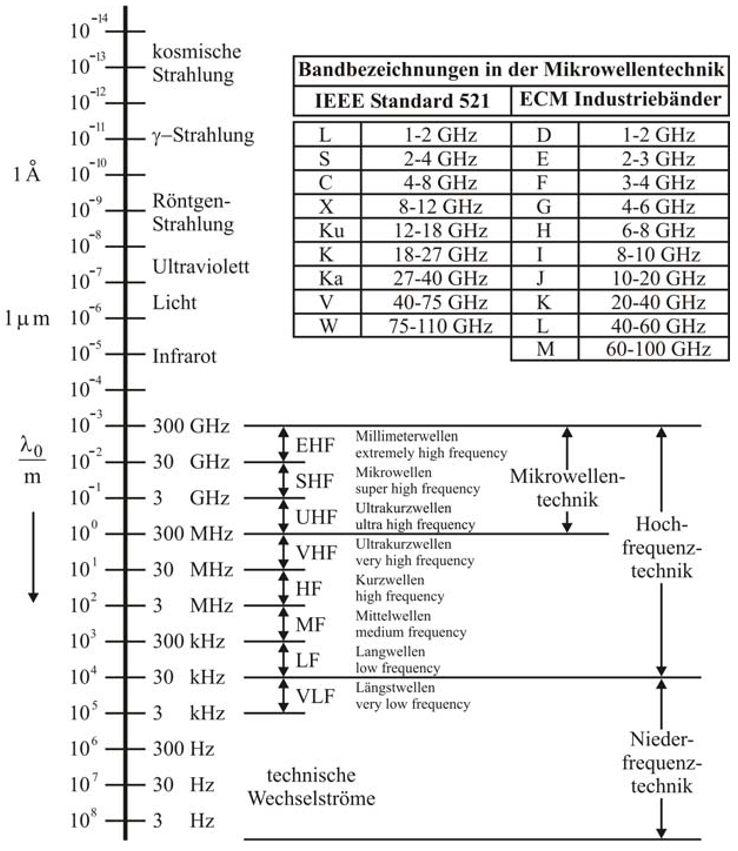
\includegraphics[width=0.75\textwidth]{frequenzbereich.png}
	\caption[Spektrum elektromagnetischer Wellen und gebräuchliche Bandbezeichnungen]{Spektrum elektromagnetischer Wellen und gebräuchliche Bandbezeichnungen. Quelle: \cite[Kark, S. 1]{Kark2006}} 
	\label{frequenzbereiche}
\end{figure}



In Deutschland gilt zudem die Aufteilung des Frequenzbereiches von 0 kHz bis 3000 GHz, welche von der Bundesnetzagentur im sogenannten Frequenzplan \cite[Bundesnetzagentur, 2016]{bundesnetzagentur-frequenzplan:2016} gemäß § 54 TKG festgehalten wird. %TODO: Was heißt "es gilt"? --> Umformulieren

\subsection{Dezimeterwelle}
Das Frequenzband von 300 MHz bis 3 GHz, auch \ac{UHF}-Band genannt, ist ein Frequenzbereich in dem die Wellen eine Länge von zehn Dezimeter bis einem Dezimeter besitzen.

\section{Bluetooth}
Bluetooth ist eine Übertragungstechnik für kabellose Kommunikation über kurze Distanzen. Es wird im Frequenzbereich von 2,4 bis 2,4835 GHz betrieben \cite[Bundesamt für Strahlenschutz, S. 1]{bundesamt-strahlungsschutz:2012}. Insgesamt gibt es unter Bluetoothgeräten drei verschiedene Sendeleistungsklassen:
\begin{description}
	\item[Klasse 1: bis 1,0 mW] Reichweite: bis 10m 
	\item [Klasse 2: bis 2,5 mW] Reichweite: 10m und mehr
	\item [Klasse 3: bis 100 mW] Reichweite: 100m und mehr
\end{description}
Die Aufteilung des Frequenzbereiches von 0 kHz bis 3000 GHz wird von der Bundesnetzagentur im sogenannten Frequenzplan \cite[Bundesnetzagentur]{bundesnetzagentur-frequenzplan:2016} gemäß § 54 TKG festgehalten.



